\documentclass[11pt,twocolumn,draft]{article}
\usepackage[T1]{fontenc}
\usepackage[
  paperwidth=21.9cm,
  paperheight=27.6cm,
  margin=1in,
  marginparwidth=0.8in,
  marginparsep=0.2in
]{geometry}
\usepackage{amsmath}
\usepackage{mathtools}
\usepackage{siunitx}
\usepackage{marginnote}
\usepackage{physics}
\usepackage{pdfpages}
\usepackage{ifdraft}
\usepackage{dirtytalk}

\usepackage{tikz}
\usepackage{pgfplots}
\pgfplotsset{compat=1.18}
\usepgfplotslibrary{fillbetween}

% For \wavyseparator
\usetikzlibrary{decorations.pathmorphing}

% For magnetic field diagrams
\usetikzlibrary{angles,quotes} % for pic (angle labels)
\usetikzlibrary{calc}
\usetikzlibrary{decorations.markings}
\tikzset{>=latex} % for LaTeX arrow head

% For arrow note
\usetikzlibrary{tikzmark,positioning}

% Arrows
\usetikzlibrary{arrows.meta}

% Links (load hyperref late to avoid conflicts)
\usepackage{hyperref}
\hypersetup{
  colorlinks=true,
  linkcolor=blue,
  urlcolor=cyan,
}

% Command for adding notes in the margin depending on single or double column layout
\makeatletter
\newcommand{\columnnote}[1]{%
  \if@twocolumn
  \if@firstcolumn
  \reversemarginpar
  \marginnote{\small\emph{#1}}%
  \normalmarginpar
  \else
  \normalmarginpar
  \marginnote{\small\emph{#1}}%
  \fi
  \else
  \marginnote{\small\emph{#1}}%
  \fi
}
\makeatother

\colorlet{Bcol}{violet!90}
\colorlet{BFcol}{red!60!black}
\colorlet{veccol}{green!45!black}
\colorlet{Icol}{blue!70!black}
\tikzset{
  BField/.style={->,very thick,Bcol},
  current/.style={->,Icol},
  force/.style={->,very thick,BFcol},
  velocity/.style={->,very thick,vcol},
  charge+/.style={very thin,draw=black,top color=red!50,bottom color=red!90!black,shading angle=20,circle,inner sep=0.5},
  charge-/.style={very thin,draw=black,top color=blue!50,bottom color=blue!80,shading angle=20,circle,inner sep=0.5},
  vector/.style={->,thick,veccol},
}
\tikzset{%
  BFieldLine/.style={thick,Bcol,decoration={markings,mark=at position #1 with {\arrow{latex}}},
  postaction={decorate}},
  BFieldLine/.default=0.5,
  pics/Bin/.style={%
    code={%
      \def\R{0.10}
      \draw[pic actions,Bcol,line width=0.6]
      (-135:\R) -- (45:\R)
      (-45:\R) -- (135:\R);
  }},
}

\newcommand{\wavyseparator}{%
  \par\vspace{0.5\baselineskip}%
  \noindent\centerline{\tikz{\draw[decorate, decoration={snake, amplitude=1mm, segment length=10mm}]
  (0,0) -- (0.8\linewidth,0);}}%
  \vspace{0.75\baselineskip}\par
}

% Make subsection counters alphabetic like in the textbook
\renewcommand\thesubsection{\thesection\Alph{subsection}}

% Customise subsection titles to show textbook page number in margin
\newcommand\mysubsection[2]{\subsection[#1]{#1\protect\columnnote{Textbook page \hyperlink{page.\number\numexpr#2+12\relax}{#2}}}}

\newcommand\seealso{\paragraph{See also}}

% document metadata
\title{Course Notes: Pearson Edexcel International A Level Physics}
\author{Luis F}
\date{\today}

\begin{document}
\maketitle
\tableofcontents
\clearpage

\section{Physics Year 1}
Consider a constant force \(\vec F\) causing a ball of mass \(m\) which is moving at a velocity \(\vec v\) to come to rest over a distance \(\vec s\).

TODO\@: TikZ diagram

Using SUVAT\@:

\begin{equation}
  v^2 = u^2 + 2as
\end{equation}

But since it comes to rest, \(v = 0\), and the initial velocity \(u = \abs{\vec v}\). Rearranging for \(a\):

\begin{align}\label{eq:proof-ke-as}
  0 &= v^2 + 2as \notag \\
  v^2 &= -2as \notag \\
  -\frac{v^2}{2} &= as \notag \\
  as &= -\frac{v^2}{2}
\end{align}

Since the work done \(W\) by a constant force is given by:

\begin{equation}
  W = \vec F \cdot \vec s = m \vec a \cdot \vec s
\end{equation}

We can substitute equation~\ref{eq:proof-ke-as} into this to get something already resembling the kinetic energy formula:

\[
  \begin{aligned}
    W &= m \cdot -\frac{v^2}{2} \\
    W &= -\frac 1 2 mv^2
  \end{aligned}
\]

Since the work done \(W\) is equal to the change in kinetic energy, and the particle ends at rest, we have:

\[
  \begin{aligned}
    W &= E_{kf} - E_{ki} \\
    W &= 0 - E_{ki} \\
    W &= -E_{ki} \\
    E_{ki} &= -W \\
    E_{ki} &= \frac 1 2 mv^2
  \end{aligned}
\]


\section{Physics Year 2}
\setcounter{section}{5}
\section{Electric and Magnetic Fields}
\setcounter{subsection}{2}
\mysubsection{Electromagnetic Effects}{56}

Gravitational, electric and magnetic fields are all vector fields. The strength of each field is defined as the force per unit something experienced by an object placed in the field:

\[
  \begin{alignedat}{3}
    \vec g                        &= \frac{\vec F} m &\qquad
    \vec E                        &= \frac{\vec F} q &\qquad
    \vec B                        &= \frac{\vec F}{q \vec v} \\[1em]
    \tikzmarknode{phiVgrav}{\Phi} &= \frac W m        &
    V                             &= \frac W q        &
    ?                             &= \frac W {q \vec v}
  \end{alignedat}
\]

\begin{tikzpicture}[remember picture, overlay]
  \node[
    font=\footnotesize
  ] (note) at ([xshift=-2em,yshift=-2em]phiVgrav)
  {Or $V_\text{grav}$};
  \draw[->, semithick] (note.north) -- (phiVgrav.south west);
\end{tikzpicture}

\wavyseparator

\[
  \begin{aligned}
    W &= \vec F \cdot \vec s \\
    W &= \abs*{\vec F}\abs*{\vec s}\cos\theta
  \end{aligned}
\]

\wavyseparator

Magnetic fields can cause circular motion!

\begin{center}
  % Adapted from https://tikz.net/magnetic_field/ by Izaak Neutelings

% B FIELD horizontal, top view, circle
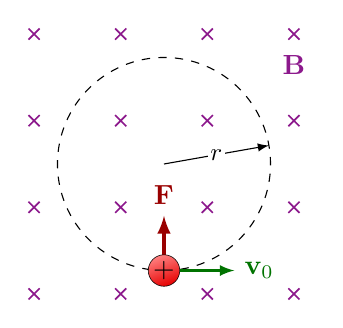
\begin{tikzpicture}
  \def\xmax{3.3}
  \def\ymax{3.3}
  \def\R{0.2}
  \def\P{0.41*\xmax}
  \def\v{0.21*\xmax}
  \def\F{0.15*\xmax}
  \def\NBy{4}
  \def\NBx{4}
  \coordinate (O) at (0.5*\xmax,0.09*\ymax+\P);
  \coordinate (Q) at (0.5*\xmax,0.09*\ymax);

  % Magnetic field
  \foreach \i [evaluate={\y=(\i-1)*\ymax/(\NBy-1);}] in {1,...,\NBy}{
    \foreach \i [evaluate={\x=(\i-1)*\xmax/(\NBx-1);}] in {1,...,\NBx}{
      \pic[rotate=-90] at (\x,\y) {Bin};
    }
  }
  \node[Bcol] at (\xmax,0.88*\ymax) {$\vb{B}$};

  % Charge
  \draw[dashed] (Q) arc (-90:270:\P) coordinate (F);
  \draw[vector] (Q)++(\R,0) --++ (\v,0) node[right] {$\vb{v}_0$};
  \draw[force]  (Q)++(0,\R) --++ (0,\F) node[above=0] {$\vb{F}$};
  \draw[charge+] (Q) circle (\R) node {$+$};
  \draw[->] (O) --++ (10:\P) node[midway,fill=white,inner sep=1,scale=0.9] {$r$};
\end{tikzpicture}

\end{center}

The forces involved are the magnetic force and the centripetal force:

\[
  \begin{alignedat}{2}
    \vec F_B &= q \vec v \cdot \vec B &\qquad
    \vec F_{cr} &= \frac{m \vec{v}^{\,2}} r
  \end{alignedat}
\]

Equating the magnetic force to the centripetal force, we can solve for the radius of the circular path:

\[
  \begin{aligned}
    q \vec v \cdot \vec B &= \frac{m \vec{v}^{\,2}} r \\
    q \vec B &= \frac{m \vec v} r \\
    r &= \frac{m \vec v}{q \vec B} \\
    r &= \frac{\vec p}{q \vec B}
  \end{aligned}
\]

\seealso
\begin{itemize}
  \item
    Raycast AI Chat, Gemini 2.5 Pro: \href{raycast://extensions/raycast/raycast-ai/ai-chat?context=%7B%22id%22:%221D3C7992-8470-4794-9406-353F68D5E439%22%7D}{%
      Electromagnetic Induction and Magnetic Forces: Equations, hints, and problem-solving
    }
\end{itemize}

\wavyseparator

Magnetic flux through an area \(A\) in a magnetic field \(B\) is given by:

\[
  \begin{aligned}
    \Phi &= \vec B \cdot \vec A \\
    \Phi &= \abs*{\vec B}\abs*{\vec A}\cos\theta
  \end{aligned}
\]

Where \(\Phi\) is in \href{https://wikipedia.org/wiki/Weber_(unit)}{webers}, \unit{\weber}, or \unit{\tesla\metre\squared}, since \(B\) is in \href{https://wikipedia.org/wiki/Tesla_(unit)}{teslas} and \(A\) is in square metres.

\wavyseparator

More magnetic flux stuff:

\[
  \begin{aligned}
    \dv t \Phi &= V \\
    \dv t N\Phi &= V
  \end{aligned}
\]

\say{The rate of change of flux linkage through a coil gives the induced e.m.f.\ across the coil.}

\begin{center}
  % B FIELD horizontal, top view, circle
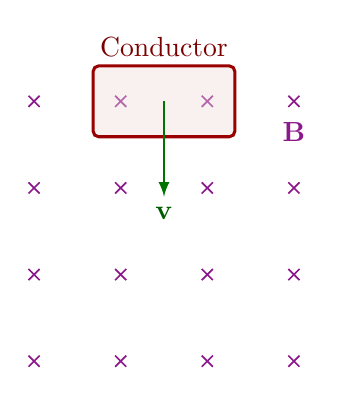
\begin{tikzpicture}
  \def\xmax{3.3}
  \def\ymax{3.3}
  \def\NBy{4}
  \def\NBx{4}

  \pgfmathsetmacro{\xstep}{\xmax/(\NBx-1)}
  \pgfmathsetmacro{\ystep}{\ymax/(\NBy-1)}

  % Magnetic field
  \foreach \i [evaluate={\y=(\i-1)*\ymax/(\NBy-1);}] in {1,...,\NBy}{
    \foreach \i [evaluate={\x=(\i-1)*\xmax/(\NBx-1);}] in {1,...,\NBx}{
      \pic[rotate=-90] at (\x,\y) {Bin};
    }
  }
  \node[Bcol] at (\xmax,0.88*\ymax) {$\vb{B}$};

  % Conductor: rectangle, positioned so it contains the top center two B field into-the-page symbols
  \coordinate (BmidL) at (\xstep, \ymax);
  \coordinate (BmidR) at (2*\xstep, \ymax);
  \def\padx{0.35}
  \def\pady{0.45}

  \draw[draw=BFcol, fill=BFcol!15, fill opacity=0.4, line width=1.1pt, rounded corners=2pt]
  ($(BmidL)+(-\padx,-\pady)$)
  rectangle
  ($(BmidR)+(\padx,\pady)$);

  \node[anchor=south, BFcol!80!black]
  at ($(BmidL)!0.5!(BmidR)+(0,\pady)$) {Conductor};

  % Motion arrow
  \draw[vector]
  ($(BmidL)!0.5!(BmidR)$)
  -- ++(0,-1.1*\ystep)
  node[below, veccol!80!black] {$\vb{v}$};
\end{tikzpicture}

\end{center}

Or we can have induction with a rotating coil in a magnetic field:

\begin{center}
  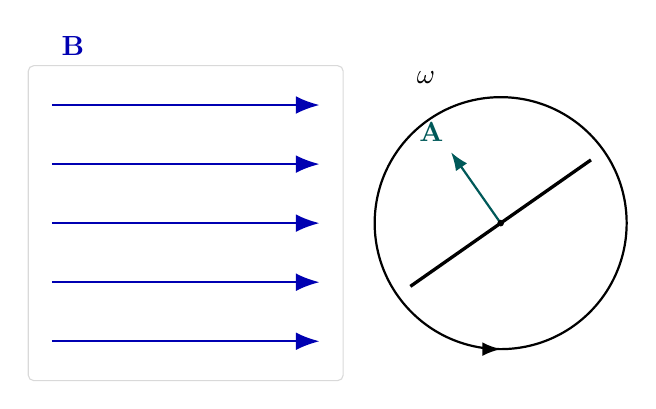
\begin{tikzpicture}[x=1cm,y=1cm]
  %--------------------------------------------
  % Styles
  %--------------------------------------------
  \tikzset{
    Bfield/.style={thick, -{Latex[length=3mm]}, blue!70!black},
    coil/.style={very thick, black},
    normalvec/.style={-Latex, thick, teal!70!black},
    rotarrow/.style={thick, postaction={decorate},
    decoration={markings, mark=at position 0.75 with {\arrow{Latex}}}}
  }

  %--------------------------------------------
  % Parameters and key points
  %--------------------------------------------
  \def\alpha{35}     % coil orientation angle (degrees from +x)
  \def\L{1.4}        % half-length of the coil line segment
  \coordinate (C) at (2,0); % center of rotation / center of coil

  %--------------------------------------------
  % Uniform magnetic field (left-to-right arrows)
  %--------------------------------------------
  % A light rectangle to suggest the uniform-field region
  \draw[rounded corners=2pt, gray!30] (-4,-2) rectangle (0,2);

  % Several horizontal arrows representing B (left -> right)
  \foreach \y in {-1.5,-0.75,0,0.75,1.5}{
    \draw[Bfield] (-3.7,\y) -- (-0.3,\y);
  }

  % Label for the magnetic field B
  \node[blue!70!black, anchor=south west] at (-3.7,2) {$\mathbf{B}$};

  %--------------------------------------------
  % Coil as a straight line (to the right of the B-field arrows)
  %--------------------------------------------
  \coordinate (P1) at ($(C)+(\alpha:\L)$);
  \coordinate (P2) at ($(C)+(\alpha+180:\L)$);
  \draw[coil] (P2) -- (P1);

  %--------------------------------------------
  % Normal vector to the coil (labeled A)
  %--------------------------------------------
  \draw[normalvec] (C) -- ++(\alpha+90:1.1)
  node[anchor=south east, xshift=1pt] {$\mathbf{A}$};

  %--------------------------------------------
  % Rotation of the coil: circular arrow labeled omega
  %--------------------------------------------
  \draw[rotarrow] (C) circle[radius=1.6];
  \node[anchor=south] at ($(C)+(120:1.9)$) {$\omega$};

  % Optional: indicate the rotation axis
  \fill (C) circle[radius=1.2pt];
\end{tikzpicture}

\end{center}

Here, e.m.f.\ is given by:

\begin{equation}\label{eq:induced-emf}
  \mathcal E = \dv t [N\Phi]
\end{equation}

Taking out the constants, rearranging and substituting:

\[
  \begin{aligned}
    \mathcal E &= N \dv{\Phi}{t} \\
    \mathcal E &= N \dv t (\vec B \cdot \vec A) \\
    \mathcal E &= N \dv t (\abs*{\vec B}\abs*{\vec A}\cos\theta)
  \end{aligned}
\]

Using \(A = \abs*{\vec A}\) and \(B = \abs*{\vec B}\) for simplicity:

\[
  \begin{aligned}
    \mathcal E &= N \dv t (BA\cos\theta) \\
    \mathcal E &= NBA \dv t [\cos\theta] \\
    \mathcal E &= NBA \dv t [\cos\omega t] \\
    \mathcal E &= -NBA \omega \sin(\omega t)
  \end{aligned}
\]

\wavyseparator

\begin{center}
  \begin{tikzpicture}
    \node (B) {$\vec B$};
    \node[above=2em of B] (IL) {$\dfrac{\vec F}{IL}$};
    \node[below left=1.4em and 2em of B] (qv) {$\dfrac{\vec F}{q\vec v}$};
    \node[below right=1.4em and 2em of B] (flux) {$\dfrac{\Phi}{\vec A}$};
    \draw[vector] (B) -- (IL);
    \draw[vector] (B) -- (qv);
    \draw[vector] (B) -- (flux);
  \end{tikzpicture}
\end{center}

Therefore,

\[
  \begin{aligned}
    \vec F &= \vec B IL \\
    \vec F &= q \vec v \cdot \vec B
  \end{aligned}
\]

\wavyseparator

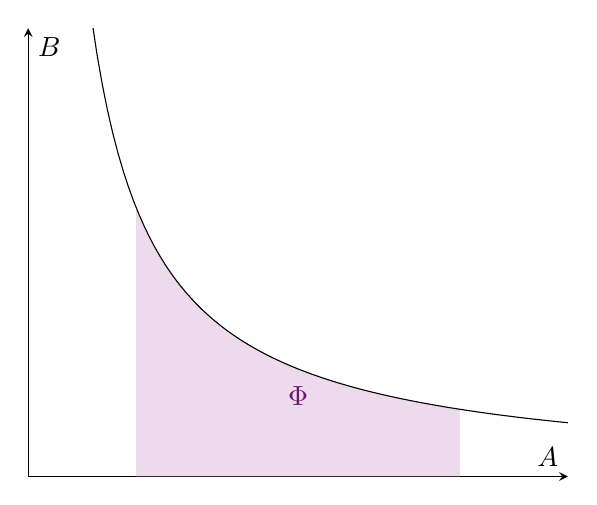
\begin{tikzpicture}
  \begin{axis}[
      xmax=5, xmin=0,
      ymax=5, ymin=0,
      axis x line=middle,
      axis y line=middle,
      samples=100,
      xtick=\empty,
      ytick=\empty,
      xlabel={$A$},
      ylabel={$B$}
    ]
    \addplot[domain=0.2:5]{3/x};
    \addplot[domain=1:4, draw=none, name path=curve]{3/x};
    \addplot[draw=none, name path=base] coordinates {(1,0) (4,0)};
    \addplot[fill=Bcol!40, fill opacity=0.4] fill between[of=curve and base];
    \node[text=Bcol!80!black] at (axis cs:2.5,0.9) {$\Phi$};
  \end{axis}
\end{tikzpicture}

\begin{tikzpicture}
  \begin{axis}[
      xmax=5, xmin=0,
      ymax=5, ymin=0,
      axis x line=middle,
      axis y line=middle,
      samples=100,
      xtick=\empty,
      ytick=\empty,
      xlabel={$t$},
      ylabel={$\Phi$}
    ]
    \addplot[domain=0.2:5]{4/x};
    \addplot[veccol, thick, domain=1.5:4.5]{8/3 - (4/9)*x};
    \addplot[mark=*] coordinates {(3,4/3)};
    \node[text=veccol!90!black, anchor=west]
    at (axis cs:2,1) {$\dv{\Phi}{t} = \mathcal E$};
  \end{axis}
\end{tikzpicture}

\wavyseparator

TRANSFORMERS!!!

Ratio of primary to secondary e.m.f.s is equal to the ratio of the number of turns in the primary to the secondary coil.

\begin{equation}\label{eq:transformer-ratios}
  \frac{\mathcal{E}_p}{\mathcal{E}_s} = \frac{N_p}{N_s}
\end{equation}

This equation can be derived using the following diagram of a transformer and the definition of e.m.f.\ seen in equation~\ref{eq:induced-emf}:

\begin{center}
  % raycast://extensions/raycast/raycast-ai/ai-chat?context=%7B%22id%22:%223C3B2520-4AD1-4099-B3D7-F9E96AA861D3%22%7D

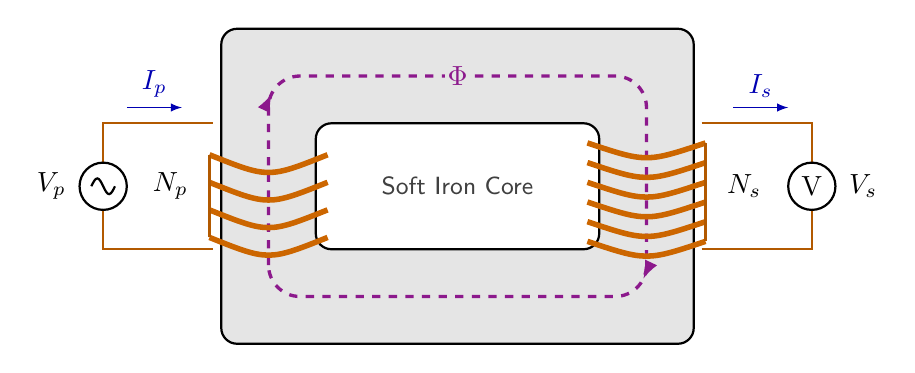
\begin{tikzpicture}
  % --- Definitions ---
  \def\coreW{6}      % Total Width
  \def\coreH{4}      % Total Height
  \def\thick{1.2}    % Iron thickness (Leg width)
  \def\holeYmin{1.2} % Bottom of hole (\thick)
  \def\holeYmax{2.8} % Top of hole (\coreH - \thick)

  % --- 1. Soft Iron Core ---
  % Drawn with even odd rule to create the hole
  \draw[fill=gray!20, draw=black, thick, rounded corners=0.2cm, even odd rule]
  (0,0) rectangle (\coreW,\coreH)
  (\thick,\thick) rectangle (\coreW-\thick, \coreH-\thick);

  \node[text=gray!50!black, font=\small\sf] at (\coreW/2, \coreH/2) {Soft Iron Core};

  % --- 2. Magnetic Flux (Phi) ---
  % Dashed path through the center of the core
  \draw[Bcol, very thick, dashed, rounded corners=0.4cm,
    decoration={markings, mark=at position 0.15 with {\arrow{latex}}, mark=at position 0.65 with {\arrow{latex}}},
  postaction={decorate}]
  (\thick/2, \thick/2) rectangle (\coreW-\thick/2, \coreH-\thick/2);

  \node[Bcol, fill=gray!20, inner sep=1pt] at (\coreW/2, \coreH-\thick/2) {$\Phi$};

  % --- 3. Primary Coil (Left Side) ---
  % Source Circuit
  \coordinate (P_top) at (0, \holeYmax);
  \coordinate (P_bot) at (0, \holeYmin);
  \coordinate (P_src) at (-1.5, 2);

  % Wires from source to coil bounds
  \draw[thick, orange!70!black] (P_src) ++(0, 0.3) -- (-1.5, \holeYmax) -- (-0.1, \holeYmax);
  \draw[thick, orange!70!black] (P_src) ++(0,-0.3) -- (-1.5, \holeYmin) -- (-0.1, \holeYmin);

  % Source Symbol (AC)
  \draw[thick, fill=white] (P_src) circle (0.3);
  \draw[thick] (P_src) ++(-0.15,0) sin ++(0.075,0.1) cos ++(0.075,-0.1) sin ++(0.075,-0.1) cos ++(0.075,0.1);
  \node[left=0.35cm] at (P_src) {$V_p$};

  % Primary Windings (fewer turns, wider spacing)
  % Constrained strictly between \holeYmin and \holeYmax
  \foreach \y in {1.35, 1.7, 2.05, 2.4} {%
    % Wire front arc: wider curve to look like it wraps around
    \draw[line width=2pt, orange!80!black] (-0.15, \y) .. controls (\thick/2, \y-0.3) .. (\thick+0.15, \y);
  }
  % Vertical schematic connector on the outside
  \draw[thick, orange!70!black] (-0.15, 1.35) -- (-0.15, 2.4);

  % Labels Primary
  \node[anchor=east] at (-0.3, \coreH/2) {$N_p$};
  \draw[current, Icol] (-1.2, \holeYmax+0.2) -- (-0.5, \holeYmax+0.2) node[midway, above] {$I_p$};

  % --- 4. Secondary Coil (Right Side) ---
  % Load Circuit
  \coordinate (S_top) at (\coreW, \holeYmax);
  \coordinate (S_bot) at (\coreW, \holeYmin);
  \coordinate (S_load) at (\coreW+1.5, 2);

  % Wires from coil to load
  \draw[thick, orange!70!black] (\coreW+0.1, \holeYmax) -- (\coreW+1.5, \holeYmax) -- (S_load) ++(0, 0.3);
  \draw[thick, orange!70!black] (\coreW+0.1, \holeYmin) -- (\coreW+1.5, \holeYmin) -- (S_load) ++(0,-0.3);

  % Load Symbol (Voltmeter)
  \draw[thick, fill=white] (S_load) circle (0.3);
  \node at (S_load) {V};
  \node[right=0.35cm] at (S_load) {$V_s$};

  % Secondary Windings (more turns, tighter spacing)
  % Constrained strictly between \holeYmin and \holeYmax
  \foreach \y in {1.3, 1.55, 1.8, 2.05, 2.3, 2.55} {%
    % Wire front arc
    \draw[line width=2pt, orange!80!black] (\coreW-\thick-0.15, \y) .. controls (\coreW-\thick/2, \y-0.25) .. (\coreW+0.15, \y);
  }
  % Vertical schematic connector on the outside
  \draw[thick, orange!70!black] (\coreW+0.15, 1.3) -- (\coreW+0.15, 2.55);

  % Labels Secondary
  \node[anchor=west] at (\coreW+0.3, \coreH/2) {$N_s$};
  \draw[current, Icol] (\coreW+0.5, \holeYmax+0.2) -- (\coreW+1.2, \holeYmax+0.2) node[midway, above] {$I_s$};

\end{tikzpicture}

\end{center}

From the diagram, we can see that the magnetic flux \(\Phi\) through each coil is the same. Therefore, we can write the e.m.f.s in each coil as:

\begin{equation}
  \mathcal{E}_p = -N_p \frac{d\Phi}{dt}, \quad \mathcal{E}_s = -N_s \frac{d\Phi}{dt}
\end{equation}

Taking the ratio of these two equations gives us equation~\ref{eq:transformer-ratios}:

\begin{equation*}
  \frac{\mathcal{E}_p}{\mathcal{E}_s} = \frac{N_p}{N_s} \tag{\ref{eq:transformer-ratios} revisited}
\end{equation*}

\section{Nuclear and Particle Physics}
\setcounter{subsection}{2}
\mysubsection{The Particle Zoo}{100}

\say{Hadrons are subatomic particles made of quarks, which experience a Strong Nuclear Force.}

\say{Quark flavour changing is done by the Weak Nuclear Force.}

\begin{center}
  % raycast://extensions/raycast/raycast-ai/ai-chat?context=%7B%22id%22:%223C3B2520-4AD1-4099-B3D7-F9E96AA861D3%22%7D

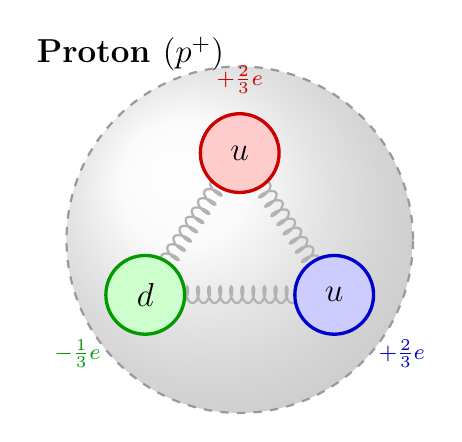
\begin{tikzpicture}
  % --- Definitions ---
  \def\R{2.2} % Radius of the proton shell

  % --- 1. The Proton Confinement (Bag) ---
  % A spherical shading to represent the particle boundary
  \shade[ball color=gray!15, opacity=0.3] (0,0) circle (\R);
  \draw[dashed, thick, gray!80] (0,0) circle (\R);

  % --- 2. Quark Positions ---
  % Equilateral triangle arrangement
  \coordinate (q1) at (0, 1.1);     % Top (Up)
  \coordinate (q2) at (1.2, -0.7);  % Bottom Right (Up)
  \coordinate (q3) at (-1.2, -0.7); % Bottom Left (Down)

  % --- 3. Gluons (Strong Force) ---
  % Drawn as springs connecting the quarks
  \begin{scope}[decoration={coil, aspect=0.4, segment length=4pt, amplitude=3pt, pre length=5pt, post length=5pt}]
    \draw[decorate, thick, gray!60] (q1) -- (q2);
    \draw[decorate, thick, gray!60] (q2) -- (q3);
    \draw[decorate, thick, gray!60] (q3) -- (q1);
  \end{scope}

  % --- 4. Quarks ---
  % Using Red, Blue, Green to subtly hint at QCD color charge,
  % though labelled by flavour (u, d).

  % Top Up Quark
  \node[circle, draw=red!80!black, fill=red!20, very thick, minimum size=1cm] (u1) at (q1) {\large $u$};
  \node[above=0.3em of u1, text=red!80!black, font=\footnotesize] {$+\frac{2}{3}e$};

  % Right Up Quark
  \node[circle, draw=blue!80!black, fill=blue!20, very thick, minimum size=1cm] (u2) at (q2) {\large $u$};
  \node[below right=0.3em of u2, text=blue!80!black, font=\footnotesize] {$+\frac{2}{3}e$};

  % Left Down Quark
  \node[circle, draw=green!60!black, fill=green!20, very thick, minimum size=1cm] (d1) at (q3) {\large $d$};
  \node[below left=0.3em of d1, text=green!60!black, font=\footnotesize] {$-\frac{1}{3}e$};

  % --- 5. Labels ---
  \node[font=\bfseries\large, anchor=north west] at (-\R-0.5, \R+0.5) {Proton $(p^+)$};
\end{tikzpicture}

  % raycast://extensions/raycast/raycast-ai/ai-chat?context=%7B%22id%22:%223C3B2520-4AD1-4099-B3D7-F9E96AA861D3%22%7D

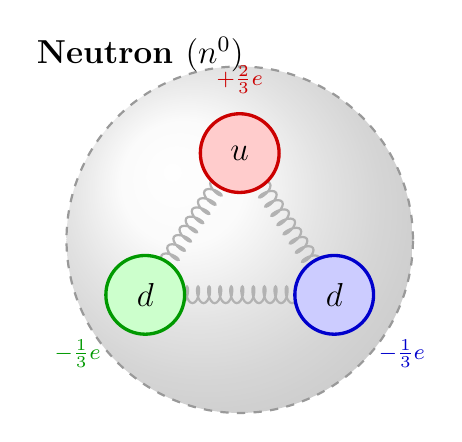
\begin{tikzpicture}
  % --- Definitions ---
  \def\R{2.2} % Radius of the neutron shell

  % --- 1. The Neutron Confinement (Bag) ---
  % A spherical shading to represent the particle boundary
  \shade[ball color=gray!15, opacity=0.3] (0,0) circle (\R);
  \draw[dashed, thick, gray!80] (0,0) circle (\R);

  % --- 2. Quark Positions ---
  % Equilateral triangle arrangement
  \coordinate (q1) at (0, 1.1);     % Top (Up)
  \coordinate (q2) at (1.2, -0.7);  % Bottom Right (Down)
  \coordinate (q3) at (-1.2, -0.7); % Bottom Left (Down)

  % --- 3. Gluons (Strong Force) ---
  % Drawn as springs connecting the quarks
  \begin{scope}[decoration={coil, aspect=0.4, segment length=4pt, amplitude=3pt, pre length=5pt, post length=5pt}]
    \draw[decorate, thick, gray!60] (q1) -- (q2);
    \draw[decorate, thick, gray!60] (q2) -- (q3);
    \draw[decorate, thick, gray!60] (q3) -- (q1);
  \end{scope}

  % --- 4. Quarks ---
  % Neutron composition: 1 Up, 2 Down (udd)
  % Colors (Red, Blue, Green) are kept to represent Color Charge neutrality.

  % Top Up Quark (Unchanged)
  \node[circle, draw=red!80!black, fill=red!20, very thick, minimum size=1cm] (u1) at (q1) {\large \(u\)};
  \node[above=0.3em of u1, text=red!80!black, font=\footnotesize] {\(+\frac{2}{3}e\)};

  % Right Down Quark (Changed from Up to Down)
  \node[circle, draw=blue!80!black, fill=blue!20, very thick, minimum size=1cm] (d1) at (q2) {\large \(d\)};
  \node[below right=0.3em of d1, text=blue!80!black, font=\footnotesize] {\(-\frac{1}{3}e\)};

  % Left Down Quark (Unchanged)
  \node[circle, draw=green!60!black, fill=green!20, very thick, minimum size=1cm] (d2) at (q3) {\large \(d\)};
  \node[below left=0.3em of d2, text=green!60!black, font=\footnotesize] {\(-\frac{1}{3}e\)};

  % --- 5. Labels ---
  \node[font=\bfseries\large, anchor=north west] at (-\R-0.5, \R+0.5) {Neutron \((n^0)\)};
\end{tikzpicture}

\end{center}

\clearpage
\appendix
\section{List of Equations}

\subsection{Waves}

\begin{itemize}
  \item \(v = \lambda f\)
  \item \(
      v^2 = \frac{
        \tikzmarknode{T}{T}
      }{
        \tikzmarknode{mu}{\mu}
      }
    \) in a uniform string/rope
\end{itemize}

\begin{tikzpicture}[remember picture, overlay]
  \node[
    font=\footnotesize
  ] (note) at ([xshift=5em,yshift=1.5em]T)
  {Force of tension};
  \draw[->, semithick] (note.south west) -- (T.north east);

  \node[
    font=\footnotesize,
    align=center
  ] (note) at ([xshift=3em,yshift=-2.5em]mu)
  {Linear density\\in \unit{\kg\per\metre}};
  \draw[->, semithick] (note.north) -- (mu.south east);
\end{tikzpicture}

\subsection{Photoelectric Effect}

\begin{itemize}
  \item \(h = \SI{6.63e-34}{\joule\second}\)
  \item \(E = hf\)
  \item \(hf = \phi + \tikzmarknode{Ekmax}{E_{k\text{max}}}\)
  \item \(V = \frac W Q \iff \tikzmarknode{W}{W} = QV\)
\end{itemize}

\begin{tikzpicture}[remember picture, overlay]
  \draw[<->, semithick]
  (Ekmax.south).. controls +(0,-1em) and +(0,1em).. (W.north);
\end{tikzpicture}


\section{List of Definitions}

\subsection{Circuits}

\begin{itemize}
  \item e.m.f.:
    \begin{itemize}
      \item Energy supplied per unit charge
      \item Work done per unit charge
      \item The work done moving unit charge around the whole circuit
    \end{itemize}
\end{itemize}


% https://steeven9.github.io/USI-LaTeX/html/math_graph.html
% https://tex.stackexchange.com/a/253040

\section{Textbook}
\ifdraft{
  The textbook pages are omitted in draft mode.
}{
  The following pages are from the Pearson Edexcel International A Level Physics Student Book 2 by Miles Hudson, and are provided here for reference. Note that some pages at the start and end are not included due to irrelevancy.

  \onecolumn
  \includepdf[pages=4-237]{textbook.pdf}
}

\end{document}
